\section{Quantum Physics}
    \subsection{Light: Particle and wave model}
        \textbf{Wave model}: double slit experiment. Light has properties of wave.

        \textbf{Particle model}: photoelectric effect. Light emit to matal and electrons emit from metal. 
    
    \subsection{Photoelectric effect}
        Light of specific range of frequency light on a metal plate and the plate emit electrons.

        \begin{figure}[H]
            \begin{center}
                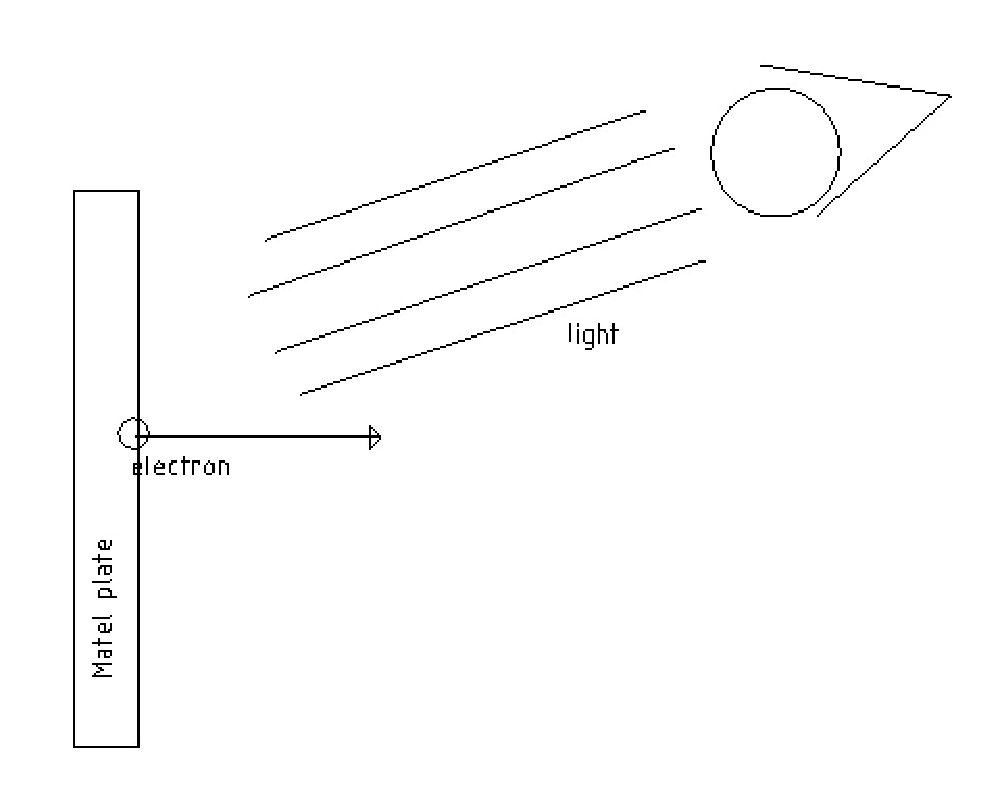
\includegraphics[height=5cm]{quantum_charts/photo_ele_show.eps}
            \end{center}
            \caption{Diagram of photoelectric effect experiment}
            \label{pe_exp_dia}
        \end{figure}

        \paragraph{Why photoelectric effect can not be explained with wave model}
            \begin{enumerate}
                \item For light with low frequency (which means low energy per photon), electrons can not emit even with long time lighting.
                        This shows energy of light can not accumulate on the electrons. 
                \item There is not time delay for electrons to emit.
                        If light is wave, it need time to transfer enough energy to emit the electrons. If light is particle, it has energy itself and can transfer its energy to electrons as it hit the electrons with no delay.
            \end{enumerate}
        
        \paragraph{Work function}
            Work function, $\phi$, is the energy required for the electron transit to ground state. It depends on the material. 

        \paragraph{Threshold frequency}
            Threshold frequency is the minimum frequency of light that can emit electrons.

            The energy of a photon with frequency $f$ is $E_p = hf$. When $E_p > \phi$, the electron emit. Thus the threshold frequency is
            \begin{align}
                f_{min} = \frac{\phi}{f}
            \end{align}

        \paragraph{Kinetic energy of emitted electron}
            Some energy of photon is used for the electrons to transit to ground state. The rest energy turns to electrons' kinetic energy. Thus the kinetic energy of the emitted electron is
            \begin{align}
                E_k = hf - \phi
            \end{align}

            This function is shown in Figure \ref{thres_freq_func}

            \begin{figure}[H]
                \begin{center}
                    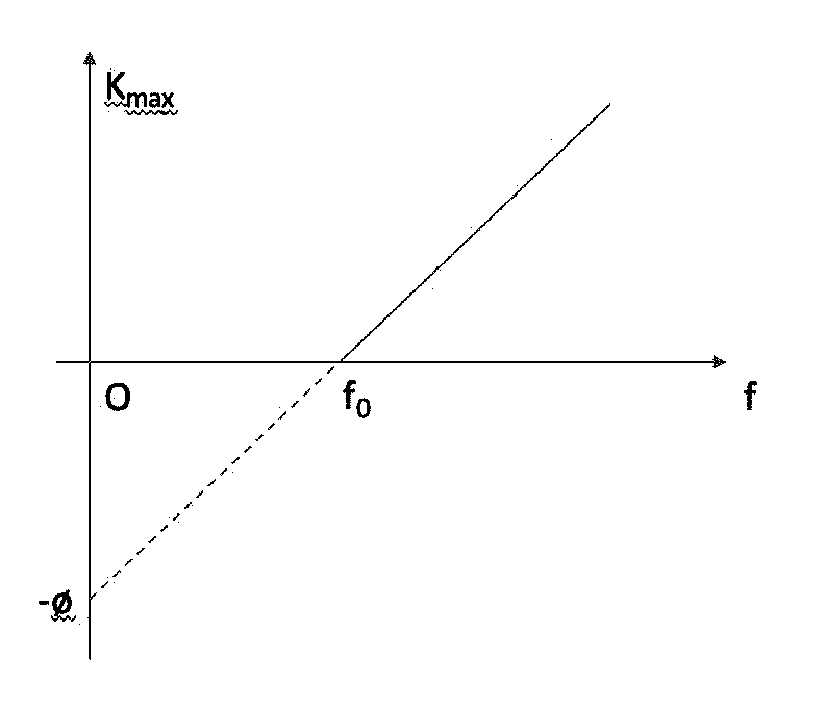
\includegraphics[height=5cm]{quantum_charts/thres_freq_func.eps}
                \end{center}
                \caption{Kinetic energy against frequency}
                \label{thres_freq_func}
            \end{figure}

        \paragraph{Photoelectric in circuit}
            Figure \ref{ph_ele_in_circ} shows a photoelectric pannel serial connected in a circuit with a cell and an ampere meter. 

            \begin{figure}[H]
                \begin{center}
                    \includegraphics[height=7cm]{quantum_charts/photo_ele_in_circ.eps}
                \end{center}
                \caption{Photoelectric experiment in circuit}
                \label{ph_ele_in_circ}
            \end{figure}

            With cell voltage $U$, the energy required for the electron to emit is $\phi + eU$. Thus the threshold frequency is $\frac{\phi + eU}{h}$

            Stop voltage, $U_0$, is when the voltage of cell that the electrons just can not emit. It is calculated by
            \begin{align}
                &\phi + eU = hf \\
                &\Rightarrow U = \frac{hf - \phi}{e}
            \end{align}

            The current in the circuit, $I$, can be calculated by
            \begin{align}
                I &= \frac{Q}{t} \\
                    &= \frac{eN}{t} \\
            \end{align}

            Here $N$ is the number of photons per second.
        
        \paragraph{Relation to the intensity of light}
            Defination of intensity: energy radiated per unit area.
            \begin{align}
                I = \frac{P}{A}
            \end{align}

            Thus, intensity of light is
            \begin{align}
                I &= \frac{P}{A} \\
                    &= \frac{\frac{N h f}{t}}{A} \\
                    &= \frac{N h f}{A t}
            \end{align}

            Thus number of photons emitted per second is
            \begin{align}
                N = \frac{I A t}{h f}
            \end{align}

            Thus, with same intensity, the higher frequency is, the smaller number of photons emitted. Photon and electron is one-to-one. Thus higher frequency is, lower current in the circuit.

    \subsection{Mass wave}
        \paragraph{Davisson Germer experiment}
            \begin{figure}[H]
                \begin{center}
                    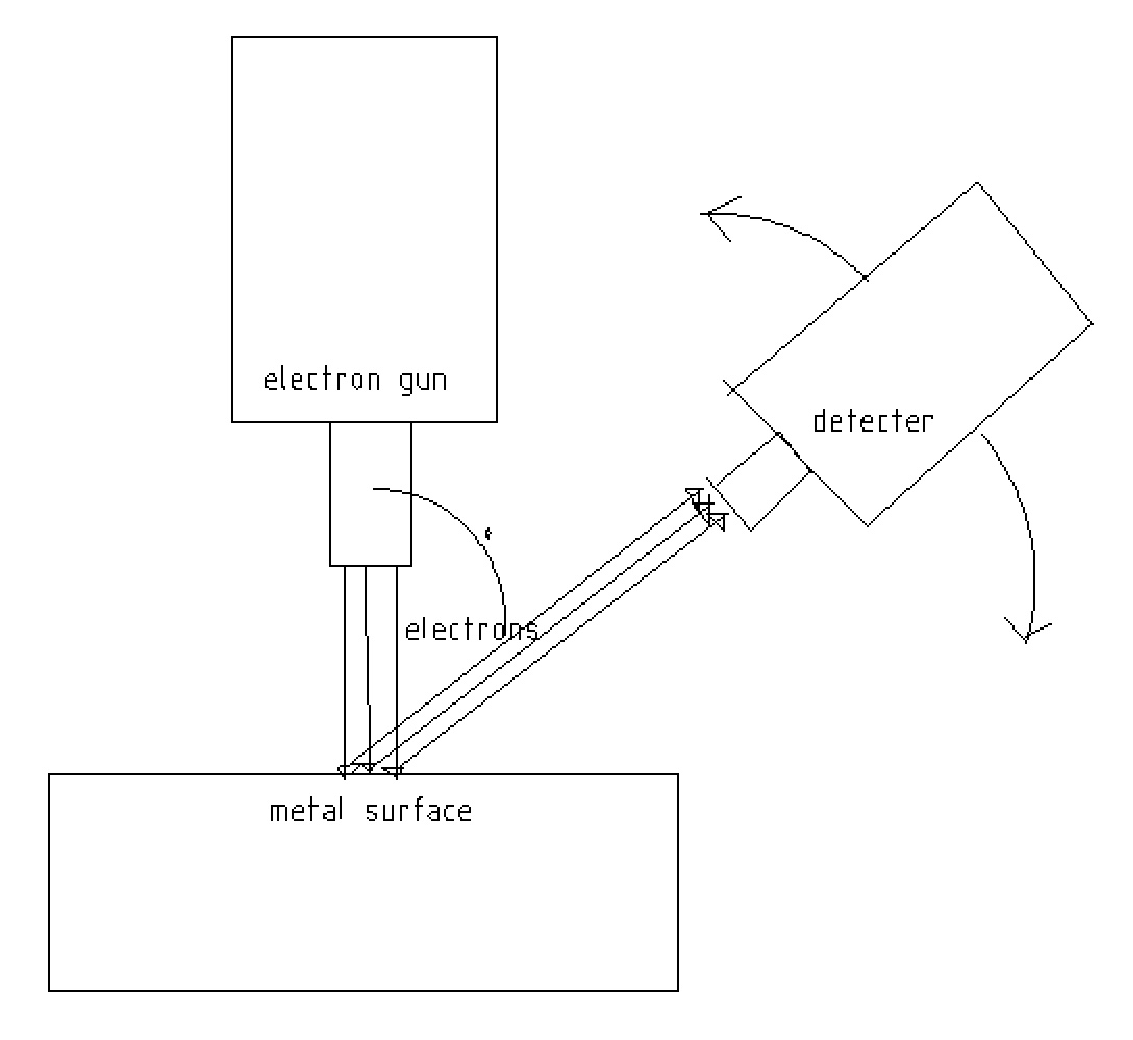
\includegraphics[height=5cm]{quantum_charts/dav_germ_exp.eps}
                \end{center}
                \caption{Davisson Germer experiment}
                \label{dav_germ_exp}
            \end{figure}

            In this experiment, change the angle between incident electrons and detecter, the intensity of electrons detected change with partern same as diffraction partern.

            This is because the electrons are diffracted by the metal lattice. This shows electrons have properties of wave.

        \paragraph{De Broglie Wave}
            De Broglie found that matter is wave. It shows probability of the position of matter. De Broglie wave length is
            \begin{align}
                \lambda = \frac{h}{p}
            \end{align}

            $h$ is the Plank constant, $p$ is the momentum of the matter.

    \subsection{Bohr model}
        


            

            